%-----------------------------------------------------------------------------
%
%               Template for LaTeX Class/Style File
%
% Name:         sigplanconf-template.tex
% Purpose:      A template for sigplanconf.cls, which is a LaTeX 2e class
%               file for SIGPLAN conference proceedings.
%
% Author:       Suresh Thummalapenta
%               Department of Computer Science
%               919 274 2896
%               sthumma@ncsu.edu
%
% Created:      27 June 2007
%
%-----------------------------------------------------------------------------


\documentclass{sigplanconf}

\usepackage{times}
\usepackage{graphicx}
\usepackage{epsf}
\usepackage{verbatim}
\usepackage{psfig}
\usepackage{cite}
\usepackage{url}
\usepackage{color}
\usepackage{alltt}

\usepackage{longtable,lscape}
\usepackage{slashbox,multirow}
\usepackage{colortbl}
\usepackage{mathrsfs}

\newcommand{\Add}{\CodeIn{add}}
\newcommand{\AVTree}{\CodeIn{AVTree}}
\newcommand{\Assignment}[3]{$\langle$ \Object{#1}, \Object{#2}, \Object{#3} $\rangle$}
\newcommand{\BinaryTreeRemove}{\CodeIn{BinaryTree\_remove}}
\newcommand{\BinaryTree}{\CodeIn{BinaryTree}}
\newcommand{\Caption}{\caption}
\newcommand{\Char}[1]{`#1'}
\newcommand{\CheckRep}{\CodeIn{checkRep}}
\newcommand{\ClassC}{\CodeIn{C}}
\newcommand{\CodeIn}[1]{{\small\texttt{#1}}}
\newcommand{\CodeOutSize}{\scriptsize}
\newcommand{\Comment}[1]{}
\newcommand{\Ensures}{\CodeIn{ensures}}
\newcommand{\ExtractMax}{\CodeIn{extractMax}}
\newcommand{\FAL}{field-ordering}
\newcommand{\FALs}{field-orderings}
\newcommand{\Fact}{observation}
\newcommand{\Get}{\CodeIn{get}}
\newcommand{\HashSet}{\CodeIn{HashSet}}
\newcommand{\HeapArray}{\CodeIn{HeapArray}}
\newcommand{\Intro}[1]{\emph{#1}}
\newcommand{\Invariant}{\CodeIn{invariant}}
\newcommand{\JUC}{\CodeIn{java.\-util.\-Collections}}
\newcommand{\JUS}{\CodeIn{java.\-util.\-Set}}
\newcommand{\JUTM}{\CodeIn{java.\-util.\-TreeMap}}
\newcommand{\JUTS}{\CodeIn{java.\-util.\-TreeSet}}
\newcommand{\JUV}{\CodeIn{java.\-util.\-Vector}}
\newcommand{\JMLPlusJUnit}{JML+JUnit}
\newcommand{\Korat}{Korat}
\newcommand{\Left}{\CodeIn{left}}
\newcommand{\Lookup}{\CodeIn{lookup}}
\newcommand{\MethM}{\CodeIn{m}}
\newcommand{\Node}[1]{\CodeIn{N}$_#1$}
\newcommand{\Null}{\CodeIn{null}}
\newcommand{\Object}[1]{\CodeIn{o}\ensuremath{_#1}}
\newcommand{\PostM}{\MethM$_{post}$}
\newcommand{\PreM}{\MethM$_{pre}$}
\newcommand{\Put}{\CodeIn{put}}
\newcommand{\Remove}{\CodeIn{remove}}
\newcommand{\RepOk}{\CodeIn{repOk}}
\newcommand{\Requires}{\CodeIn{requires}}
\newcommand{\Reverse}{\CodeIn{reverse}}
\newcommand{\Right}{\CodeIn{right}}
\newcommand{\Root}{\CodeIn{root}}
\newcommand{\Set}{\CodeIn{set}}
\newcommand{\State}[1]{2^{#1}}
\newcommand{\TestEra}{TestEra}
\newcommand{\TreeMap}{\CodeIn{TreeMap}}

\newenvironment{CodeOut}{\begin{scriptsize}}{\end{scriptsize}}
\newenvironment{SmallOut}{\begin{small}}{\end{small}}

\newcommand{\pairwiseEquals}{PairwiseEquals}
\newcommand{\monitorEquals}{MonitorEquals}
%\newcommand{\monitorWField}{WholeStateW}
\newcommand{\traverseField}{WholeState}
\newcommand{\monitorSMSeq}{ModifyingSeq}
\newcommand{\monitorSeq}{WholeSeq}

\newcommand{\IntStack}{\CodeIn{IntStack}}
\newcommand{\UBStack}{\CodeIn{UBStack}}
\newcommand{\BSet}{\CodeIn{BSet}}
\newcommand{\BBag}{\CodeIn{BBag}}
\newcommand{\ShoppingCart}{\CodeIn{ShoppingCart}}
\newcommand{\BankAccount}{\CodeIn{BankAccount}}
\newcommand{\BinarySearchTree}{\CodeIn{BinarySearchTree}}
\newcommand{\LinkedList}{\CodeIn{LinkedList}}

\newcommand{\Book}{\CodeIn{Book}}
\newcommand{\Library}{\CodeIn{Library}}

\newcommand{\Jtest}{Jtest}
\newcommand{\JCrasher}{JCrasher}
\newcommand{\Daikon}{Daikon}
\newcommand{\JUnit}{JUnit}

\newcommand{\trie}{trie}

\newcommand{\Perl}{Perl}


\newcommand{\SubjectCount}{11}
\newcommand{\DSSubjectCount}{two}

\newcommand{\Equals}{\CodeIn{equals}}
\newcommand{\Pairwise}{PairwiseEquals}
\newcommand{\Subgraph}{MonitorEquals}
\newcommand{\Concrete}{WholeState}
\newcommand{\ModSeq}{ModifyingSeq}
\newcommand{\Seq}{WholeSeq}
\newcommand{\Aeq}{equality}

\newcommand{\Meaning}[1]{\ensuremath{[\![}#1\ensuremath{]\!]}}
\newcommand{\Pair}[2]{\ensuremath{\langle #1, #2 \rangle}}
\newcommand{\Triple}[3]{\ensuremath{\langle #1, #2, #3 \rangle}}
\newcommand{\SetSuch}[2]{\ensuremath{\{ #1 | #2 \}}}

\newcommand{\Equiv}[2]{\ensuremath{#1 \EquivSTRel{} #2}}
\newcommand{\EquivME}{\Equiv}
\newcommand{\EquivST}{\Equiv}
\newcommand{\EquivSTRel}{\ensuremath{\cong}}
\newcommand{\Redundant}[2]{\ensuremath{#1 \lhd #2}}
\newcommand{\VB}{\ensuremath{\mid}}
\newcommand{\MES}{method-entry state}

\newcommand{\Small}[1]{{\small{#1}}}

\newcommand{\CenterCell}[1]{\multicolumn{1}{c|}{#1}}
 
\usepackage{amsmath}


\begin{document}

\conferenceinfo{OOPSLA}{'07 Montreal, Canada}
\copyrightyear{200X} 
\copyrightdata{X-XXXXX-XX-X/XX/XX} 

%\titlebanner{banner above paper title}        % These are ignored unless
%\preprintfooter{short description of paper}   % 'preprint' option specified.

\title{Exploiting Code Search Engines to Improve Programmer Productivity}

\authorinfo{Suresh Thummalapenta}
           {Department of Computer Science\\North Carolina State University\\Raleigh, USA}
           {sthumma@ncsu.edu}
\maketitle

\begin{abstract}

Software developers often face
challenges in reusing open source frameworks due to several factors
such as the framework complexity and lack of proper
documentation. In this paper, we propose a code-search-engine-based
approach that detects \Intro{hotspots} in a given framework
by mining code examples gathered from open source repositories available on the web; 
these hotspots are API classes and methods that are frequently reused. 
Hotspots can serve as starting points for developers
in understanding and reusing the given framework. 
Our approach also detects \Intro{coldspots}, which are API classes and methods that are rarely used.
Coldspots serve as caveats for developers as there can 
be difficulties in finding relevant code examples and are generally less exercised
compared to hotspots. We developed a tool, called SpotWeb, for
frameworks or libraries written in Java and used our tool
to detect hotspots and coldspots of eight widely used open source
frameworks. We show the utility of our detected hotspots 
by comparing these hotspots with the API classes reused by a real application
and compare our results with the results of a previous related approach.
\end{abstract}


\category{D.2.3}{Software Engineering}{Coding Tools and Techniques}[Object-oriented programming] 
{\bf General Terms:} Languages, Experimentation.\\
{\bf Keywords:} Code reuse, Code search engine, Code examples, hotspots


\section{Introduction}
\label{sec:intro}
\vspace*{-3ex}
Programming languages such as Java and C++ provide exception-handling 
constructs such as \CodeIn{try-catch} to handle exception conditions that arise
during program execution. Under these exception conditions, programs follow paths
different from normal execution paths; these additional paths are referred to as 
\emph{exception} paths. Applications developed based on these programming
languages are expected to handle these exception conditions and take necessary recovery
actions. For example, when an application reuses resources such as files or database connections,
the application should release the resources after the usage in all paths
including \Intro{exception} paths. Failing to release the resources can not only cause performance degradation, 
but can also lead to critical issues. For example, if a database lock acquired by a
process is not released, any other process trying to acquire the same lock
hangs till the database releases the lock after timeout.
A case study~\cite{Weimer04} conducted on a real application 
demonstrates the necessity of releasing resources in exception paths 
for improving reliability and performance. 
The case study found that there was a surprising
improvement of 17\% in performance of the application after 
correctly releasing resources in the presence of exceptions.

\Comment{In general, software verification concentrates on verifying behaviors of the application 
during normal execution paths rather than exception paths. Therefore, the exception 
cases remain undetected during traditional software verification.}

Software verification can be challenging for exception cases as verification
techniques require specifications that describe expected behaviors when exceptions occur.
These specifications are often not available in practice~\cite{document:leth}.
To address this issue, association rules of the form ``$FC_a$ $\Rightarrow$ $FC_e$''
are mined as specifications~\cite{WeimerN05}, where both $FC_a$ and $FC_e$ are function calls that share
the same receiver object. These specifications are used to 
verify whether the function call $FC_a$ is followed by the function call $FC_e$ in all 
exception paths. However, simple association rules of this form are often not sufficient
to characterize common exception-handling rules. The rationale is that
there are various scenarios where $FC_a$ is not necessarily followed by $FC_e$ 
when exceptions are raised by $FC_a$, although both function calls 
share the same receiver object. 

\begin{figure*}[t]
\centering
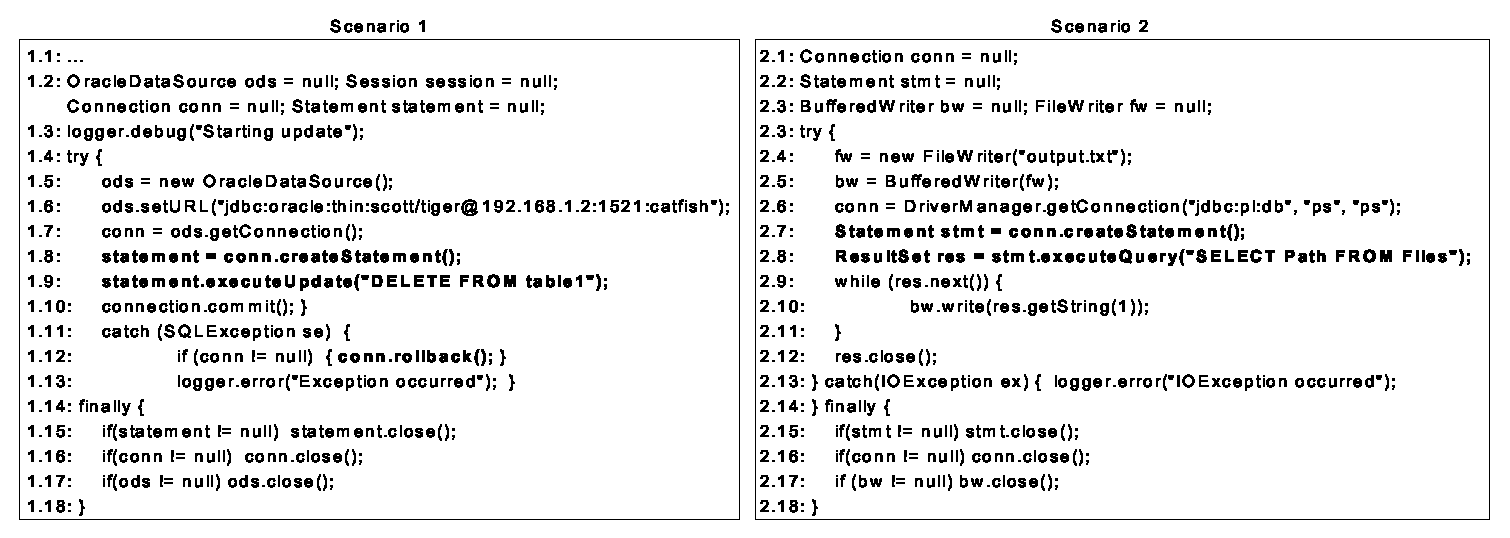
\includegraphics[scale=0.70,clip]{figs/three-code-examples1.eps}\vspace*{-3ex}
\centering \caption {\label{fig:threescenarios} Two example scenarios from real applications.}\vspace*{-4ex}
\end{figure*}

We next present an example using Scenarios 1 and 2 (extracted 
from real applications) shown in Figure~\ref{fig:threescenarios}. 
Scenario 1 attempts to modify contents of a database through the function call
\CodeIn{Statement.executeUpdate} (Line 1.9), whereas Scenario 2 attempts to read contents
of a database through the function call \CodeIn{Statement.executeQuery} (Line 2.8).
Consider a simple specification in the form of an association
rule ``\CodeIn{Connection creation} $\Rightarrow$
\CodeIn{Connection rollback}''. This rule describes that a \CodeIn{rollback} function call should
appear in exception paths whenever an object of \CodeIn{Connection} is created. 
Although a \CodeIn{Connection} object is created in both
scenarios, this rule applies only to Scenario 1 and does not apply to Scenario 2.
The primary reason is that the \CodeIn{rollback} function call should be invoked \emph{only} when 
there are any changes made to the database. This example shows that
simple association rules of the form ``$FC_a$ $\Rightarrow$ $FC_e$''
are often insufficient to characterize exception-handling rules.

The insufficiency of simple association rules calls for 
more general association rules, hereby referred to as \Intro{sequence association rules},
of the form ``($FC_c^1$...$FC_c^n$) $\wedge$ $FC_a$ $\Rightarrow$ ($FC_e^1$...$FC_e^m$)''.
This sequence association rule describes that function call $FC_a$ should be followed 
by function-call sequence $FC_e^1$...$FC_e^m$ in exception paths only 
when preceded by function-call sequence $FC_c^1$...$FC_c^n$. Using this sequence association rule,
the preceding example can be expressed as ``($FC_c^1$$FC_c^2$) $\wedge$ 
$FC_a$ $\Rightarrow$ ($FC_e^1$)'', where

$FC_c^1$ : \CodeIn{OracleDataSource.getConnection}\\
\hspace*{0.15in}$FC_c^2$ : \CodeIn{Connection.createStatement}\\
\hspace*{0.15in}$FC_a$ : \CodeIn{Statement.executeUpdate}\\
\hspace*{0.15in}$FC_e^1$ : \CodeIn{Connection.rollback}\\
\vspace*{-2ex}

This sequence association rule applies to Scenario 1 and
does not apply to Scenario 2 due to the presence of $FC_a$: \CodeIn{Statement.executeUpdate}.
The key aspects to be noted in this rule are: (1) \CodeIn{Statement.executeUpdate}
is the primary reason to have \CodeIn{Connection.rollback} in an exception path and
(2) the receiver object of \CodeIn{Statement.executeUpdate} is dependent on the 
receiver object of \CodeIn{Connection.rollback} through the function-call sequence
defined by $FC_c^1$$FC_c^2$.

Our sequence association rules are a super set of simple association rules.
For example, sequence association rules are the same as simple association
rules when the sequence $FC_c^1$...$FC_c^n$ is empty. 
To the best of our knowledge, existing association rule mining techniques~\cite{agarwal:association}
cannot be directly applied to mine these sequence association rules. 
Therefore, to bridge the gap, we develop a new mining algorithm by adapting the
frequent closed subsequence mining technique~\cite{wang:bide}. 

We further develop a novel approach, called CAR-Miner, that incorporates
our new mining algorithm for the problem of detecting exception-handling rules in
the form of sequence association rules by analyzing source code. Apart from mining sequence
association rules, CAR-Miner addresses another challenge that is often faced 
by existing approaches~\cite{Zhenmin2005PRMiner, chang07:finding, WeimerN05}, 
which mine rules from a limited data scope, 
i.e., from only a few example applications. Therefore, these approaches may not 
be able to mine rules that do not have enough
supporting samples in those example applications, and hence 
the related defects remain undetected by these approaches. To address
this challenge, CAR-Miner expands the data scope by leveraging a code search engine (CSE)
for gathering relevant code samples from existing open source projects available
on the web. From these relevant code samples, CAR-Miner mines exception-handling rules. 
We show the usefulness of mined exception-handling rules
by applying these rules on five applications to detect violations.
CAR-Miner tries to address problems related to the quality of code samples 
gathered from a CSE by capturing the most frequent patterns through mining.

\Comment{In particular, CAR-Miner accepts an input application and tries to detect
exception-handling defects in that application. Initially, CAR-Miner gathers function calls, referred as
$FC_a$, used by  the input application. CAR-Miner interacts with a code search engine (CSE) such as Google code search~\cite{GCSE} to gather related code examples that are already reusing $FC_a$. 
CAR-Miner constructs an Exception Flow Graph (EFG) for each code example gathered from 
the CSE. EFG is an extended form of control flow graph that captures flow of control in both
normal and exception conditions. While constructing EFG, we add only those exception
paths that can occur potentially during program execution. To capture such
exception paths, we use a sound static analysis that provides a set
of exceptions thrown by each $FC_a$ during program execution. 
CAR-Miner collects traces, which are
in the form of a sequence of function calls, from EFG post-processes these 
traces to filter unrelated function calls of $FC_a$.
CAR-Miner mines these traces to capture sequence association rules. 
Finally, CAR-Miner applies mined exception-handling rules to detect violations in the input application.
As CAR-Miner leverages a code search engine for gathering related code examples,
CAR-Miner has an added advantage of being able to mine rules, which do not have enough
supporting samples in the input application. CAR-Miner tries to address the 
problems related to the quality of the code examples 
gathered from a CSE by capturing the most frequent rule candidates through mining.}

This paper makes the following main contributions:\vspace*{-1ex}
\begin{Itemize}
\item A general mining algorithm to mine sequence association rules of the form 
``($FC_c^1$...$FC_c^n$) $\wedge$ $FC_a$ $\Rightarrow$ ($FC_e^1$...$FC_e^m$)''.
Our new mining algorithm takes a step forward in the direction 
of developing new mining algorithms to address
unique requirements in mining software engineering data, beyond being limited
by existing off-the-shelf mining algorithms.\vspace*{-2ex}
\item An approach that incorporates the general mining algorithm to mine exception-handling
rules that describe expected behavior when exceptions occur during
program execution. \vspace*{-2ex}
\item A technique for constructing a precise Exception-Flow Graph (EFG), which is an extended form of 
a Control-Flow Graph (CFG), that includes only those exception paths that can potentially occur 
during program execution.\vspace*{-2ex}
\item An implementation for expanding the data scope to open source projects that help
detect new related exception-handling rules that do not have enough supporting samples in an application under analysis.
These rules can help detect new defects in the application under analysis.\vspace*{-2ex}
\item Two evaluations to show
the effectiveness of our approach. (1) CAR-Miner detects $294$ real 
exception-handling rules in five different applications including $285$ KLOC. 
(2) The top $50$ exception-handling
rules (top $10$ real rules of each application)
are used to detect a total of $160$ real defects in these five
applications, where $87$ defects are new, not being detected by a 
previous related approach~\cite{WeimerN05}. \Comment{The initial response from 
developers of HsqlDB~\footnote{\url{http://hsqldb.sourceforge.net/}} is
encouraging. The developers responded on the first ten defects that we reported, 
where seven defects are \emph{accepted} and only three defects are rejected.}
\end{Itemize}

The rest of the paper is organized as follows. 
%Section~\ref{sec:example} presents example scenarios.
Section~\ref{sec:condrules} presents a formal definition of sequence
association rules and describes our new mining algorithm.
Section~\ref{sec:approach} describes key aspects of the CAR-Miner approach.
Section~\ref{sec:eval} presents evaluation results.
%Section~\ref{sec:discussion} presents limitations and future work.
Section~\ref{sec:threats} discusses threats to validity.
Section~\ref{sec:related} presents related work.
Finally, Section~\ref{sec:conclusion} concludes.



%-------------------------------------------------------------------------------
\section{Framework}
\label{sec:framework}

Our framework consists of three major components: the code downloader,
code search engine, and code analyzer. Figure~\ref{fig:architecture}
shows an overview of all components and flows among different components.

\begin{figure}[t]
\centering
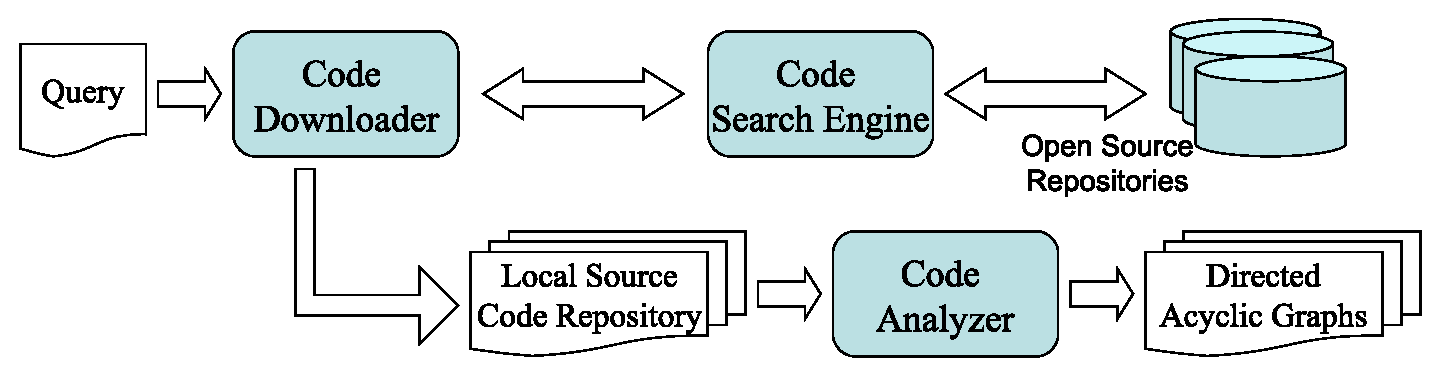
\includegraphics[scale=0.36,clip]{Framework1.eps}
\caption{Overview of the framework} \label{fig:architecture}
\vspace*{-2ex}
\end{figure}

Given a query, the code downloader interacts with a CSE and downloads
relevant code samples. The downloaded code samples, which are partial, form a local
source code repository that serves as input to the code analyzer.
The code analyzer performs static analysis over each code sample with heuristics and
transforms the sample into an intermediate form represented as a DAG.
During transformation, statements inside loops like \emph{while} and \emph{for}
are treated as a group of statements that are executed either once or not.
While constructing DAG, the code analyzer also performs method inlining
by replacing method invocations of the current class with the
body of the corresponding method declarations. Each node in the constructed
DAG represents a statement in the code sample. During transformation,
the code analyzer uses several heuristics to gather additional type information
for each statement. For example, the additional type information for
a method-invocation statement includes the receiver object type, the
return object type, and argument types. We explain a heuristic
used in our framework through the code sample shown below:

\begin{CodeOut}
\begin{alltt}
\textbf{public} QueueSession test()\hspace*{0.2in}\{ ...
\hspace*{0.4in}\textbf{return} connect.createQueueSession(false,int);\}
\end{alltt}
\end{CodeOut}
\vspace*{-1ex}

In this code sample, the method-invocation
\CodeIn{createQueueSession} is a part of the return statement. The
receiver object type of method-invocation
\CodeIn{createQueueSession} can be inferred by looking up the
declaration of the \CodeIn{connect} variable. But as our framework
deals with the code sample that is partial, it is difficult to get
the return type of the method-invocation with out being able to
access the corresponding method declaration in the downloaded file.
However, the return type can still be inferred from the return type
of the enclosing method declaration. As the enclosing method
declaration has return type \CodeIn{QueueSession}, we can infer that
the return type of the method-invocation \CodeIn{createQueueSession}
is \CodeIn{QueueSession} or one of its subtypes. In our framework
implementation, we used GCSE as an underlying CSE.
%-------------------------------------------------------------------------------
\section{Tools}
\label{sec:extensions}

We developed two tools by extending our described framework. The results of these tools
show the effectiveness of our framework.
\Comment{PARSEWeb takes queries of the form ``\emph{Source Object Type} $\rightarrow$
\emph{Destination Object Type}'' as input and suggests frequent method-invocation
sequences that can take the \emph{Source Object Type} as input
and result in the \emph{Destination Object Type}. The second tool, called Hotspotter,
extends the described framework for identifying usage hotspots and weakspots in the library or framework given as input.}
%-------------------------------------------------------------------------------
\subsection{PARSEWeb}
\label{sec:parseweb}

\begin{figure}[t]
\centering
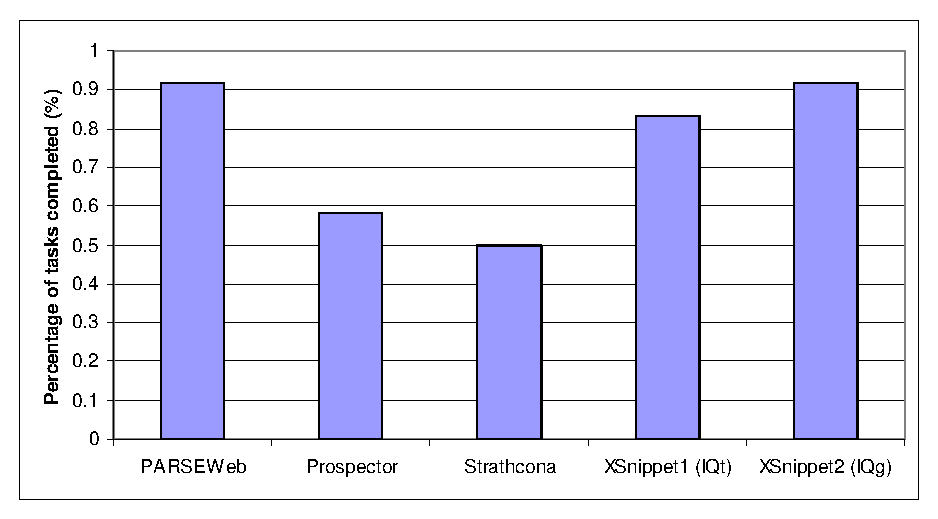
\includegraphics[scale=0.50,clip]{ComparisonResults1.eps}
\caption{Evaluation results of PARSEWeb with related tools Prospector, Strathcona, and XSnippet} \label{fig:comparison}
\vspace*{-2ex}
\end{figure}
A common problem faced by programmers while reusing existing
frameworks or libraries is that the programmers often know what type
of object that they need, but do not know how to get that object
with a specific method sequence. We developed PARSEWeb to address
the preceding issue. PARSEWeb\footnote{Available at
\url{http://ase.csc.ncsu.edu/parseweb/}} accepts a query of the form
``\emph{Source} $\rightarrow$ \emph{Destination}'', and gives the
\emph{Source} and \emph{Destination} object types as input to the
described framework, which in turn provides graphs (DAG) for each
downloaded code sample as output. PARSEWeb identifies nodes that
contain the given \emph{Source} and \emph{Destination} object types
as Source and Destination nodes, respectively. PARSEWeb extracts a
method-invocation sequence by calculating the shortest path between
Source and Destination nodes. We evaluated PARSEWeb with related
existing tools Prospector~\cite{prospector:jungloid},
Strathcona~\cite{strathcona:se}, and XSnippet~\cite{xsnippet:saha}
for 12 specific programming tasks taken from the XSnippet approach.
The results of our evaluation are shown in
Figure~\ref{fig:comparison}. The XSnippet1 and XSnippet2 entries
show results with two query-type techniques $IQ_{T}$ and $IQ_{G}$ of
XSnippet, respectively. PARSEWeb performed better than Prospector,
Strathcona, and XSnippet1. The results of PARSEWeb are at par with
XSnippet2. Moreover, as PARSEWeb is developed based on our framework
that uses CSEs for gathering relevant code samples on demand, unlike
other related tools, PARSEWeb is not limited to the queries of any
specific set of frameworks or libraries. \Comment{The results
signify the effectiveness of the underlying framework used by
PARSEWeb. $IQ_{G}$ query type (XSnippet2). However, the
``XSnippet2'' cannot effectively address the issue targeted by
PARSEWeb as this query type simply returns the set of all code
samples contained in the sample repository that instantiate the
given \emph{Destination} object type, irrespective of the
\emph{Source} object type.}

%-------------------------------------------------------------------------------
\subsection{Hotspotter}
\label{sec:hotspotter}

\setlength{\tabcolsep}{1pt}
\begin{table}[t]
\begin{SmallOut}
\begin{CodeOut}
\begin{center}
\begin {tabular} {|c|l|c|c|c|c|c|c|c|}
\hline
S.No.&Subject&Total&\multicolumn{2}{|c|}{Hotspots}&\multicolumn{2}{|c|}{Weakspots}&\multicolumn{2}{|c|}{Deadspots}\\
\cline{4-9}
&Name&No. of APIs&No.&\%&No.&\%&No.&\%\\
\hline 1&JUnit&379&22&5.8&83&21.9&124&32.7\\
\hline 2&Log4j&1334&21&1.6&180&13.5&746&55.9\\
\hline 3&BCEL&2691&18&0.7&486&18.1&1867&69.4\\
\hline 4&Struts&4679&28&0.6&0&0&4332&92.6\\
\hline
\end{tabular}
\centering \caption {\label{tab:hotspotterresults} Evaluation results
 of Hotspotter with four subjects}
\centering {\CodeIn{Total: Total number of APIs, No.: Number of APIs identified as hotspots, weakspots, and deadspots
and their percentage (shown with \%) among the total number of APIs.}}
\end{center}
\end{CodeOut}
\end{SmallOut}
\vspace*{-4ex}
\end{table}
Object-oriented frameworks are designed mainly with the concern of
reusability. Framework users, who develop concrete applications by
customizing frameworks, must be aware of its areas of flexibility
that are commonly referred as hotspots. We developed Hotspotter for
identifying hotspots in a given input framework. These hotspots can
serve as a starting point for users of the input framework.
Hotspotter also assists framework developers by identifying
weakspots and deadspots. Weakspots are APIs that are rarely used and
deadspots are APIs that are not used among the samples gathered from
CSEs. These weakspots and deadspots can help developers to analyze
whether to keep those APIs in further versions or whether the
functionality provided by those APIs is subsumed by other APIs.

Hotspotter identifies hotspots, weakspots, and deadspots in the given input framework by
calculating the Usage Percentage (\emph{UP}) of each public or protected API among
the code samples returned by the CSE. The \emph{UP} of an API is calculated as
(\CodeIn{No. of usages of the API} / \CodeIn{Total no. of usages of all APIs}) * 100.
Hotspotter uses two threshold values: Upper Threshold (\emph{UTH}) and Lower Threshold (\emph{LTH}).
APIs with \emph{UP} more than \emph{UTH} are classified
as hotspots and APIs with \emph{UP} less than \emph{LTH} and greater than zero are classified as weakspots.
APIs with \emph{UP} of zero are classified as deadspots.
In our implementation, we used \emph{UTH} value as 1\% and \emph{LTH} value as 0.1\%.
We plan to find optimum values for these parameters by
analyzing other open source frameworks. Table~\ref{tab:hotspotterresults} shows
preliminary results of Hotspotter with four subject frameworks JUnit, Log4j,
BCEL, and Struts. Our results show that the framework users often use only a small subset of the
total number of APIs provided by the framework. \Comment{To further assist framework users,
Hotspotter sorts the final results and gives the most frequently used hotspot.
For example, Hotspotter gave the API \CodeIn{org.apache.log4j.Logger,getLogger(java.lang.String)} as the most
frequently used hotspot of the Log4j framework.}\Comment{This API is already known to be the most relevant API
for users of the Log4j framework.}

\section{Conclusion}
\label{sec:conclusion}

Mapping relations of APIs are quite useful for the translation
of projects from one language to another language, and
it is difficult to mine these mapping relations due to various
challenges. In this paper, we propose a novel approach that mines mapping
relations of APIs from existing projects with multiple versions in
different languages. We conducted two evaluations to show the effectiveness
of our approach. The results show that our approach mines many API mapping
relations between Java and C\#, and these relations improve existing language
translation tools such as Java2CSharp.

\bibliographystyle{abbrv}
\bibliography{sthumma-oopslasrc07}
\end{document}
